\documentclass{beamer}

\setbeamertemplate{navigation symbols}{}
\setbeamertemplate{footline}[page number]
\setbeamertemplate{caption}[numbered]

\usepackage{amsmath}

\usefonttheme[mathonly]{serif}
\usepackage[lf]{venturis}
\setbeamerfont{footnote}{size=\tiny}
\setbeamerfont{caption}{size=\scriptsize}


\title{\textbf{Detectors and Methods for QGP Measurements}}
\author{Shih-Kai Lin}
\institute{University of Houston}
\date{2013 December 12}

\begin{document}

\begin{frame}
\titlepage
\end{frame}


\begin{frame}{outline}
	\begin{itemize}
	\item a heuristic derivation of Bethe's formula
	\item particle identification
	\item centrality measurement
	\item temperature measurement
	\end{itemize}
\end{frame}


\begin{frame}{Bethe's formula: a heuristic derivation\footnote{From J.D. Jackson's classical textbook, \textit{Classical Electrodynamics}}}
Bethe's formula in its simpler form
\begin{equation}
-\frac{dE}{dx}=\frac{2\pi NZz^2e^4}{mc^2\beta^2}\left( \ln\left( \frac{2\gamma^2\beta^2mc^2}{I} \right) -\beta^2\right)
\end{equation}

\begin{table}
\scriptsize
\begin{tabular}{rl}
	$N$ & : number of atoms per unit volume \\
	$Z$ & : number of electrons per atom \\
	$ze$ & : charge of incident particle \\
	$m$ & : electron mass \\
	$\beta$ & : speed of incident particle \\
	$I$ & : mean ionization potential
\end{tabular}
\end{table}

\textcolor{red}{idea}: transform to the rest frame of the incident particle and approximate it as a fixed charge center.
\end{frame}


\begin{frame}{Mott scattering}
\begin{columns}
	\begin{column}{0.2\textwidth}
		\begin{figure}
			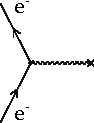
\includegraphics[width=\textwidth]{plots/Mott_Feyn.pdf}
		\end{figure}
	\end{column}
	\begin{column}{0.8\textwidth}
	\begin{itemize}
	\item	differential scattering cross-section
		\begin{equation}
		\frac{d\sigma}{d\Omega}=\left( \frac{ze^2}{2pv} \right)^2 \frac{1}{\sin^4\frac{\theta}{2}} \left( 1-\beta^2\sin^2\frac{\theta}{2} \right)
		\end{equation}
	\item rewrite it as a function of energy gain of the electron $T$($=$ energy loss of the incident particle) in the electron rest frame
		\begin{equation*}
		\frac{d\sigma}{d\Omega}\leftrightarrow \frac{d\sigma}{dQ^2}\leftrightarrow \frac{d\sigma}{dT}
		\end{equation*}
		
	\item	therefore
		\begin{equation}
		\frac{d\sigma}{dT}=\left( \frac{2\pi z^2e^4}{mc^2\beta^2T^2} \right)\left( 1-\beta^2\frac{T}{T_{max}} \right)
		\end{equation}
	\end{itemize}
	\end{column}
\end{columns}

\end{frame}



\begin{frame}{maximum energy transfer}
\begin{itemize}
\item energy loss per unit length can be obtained by
\begin{equation}
-\frac{dE}{dx}=\int_I^{T_{max}}T\times \textcolor{red}{NZ\frac{d\sigma}{dT}dT}=\frac{2\pi NZz^2e^4}{mc^2\beta^2}\left(\ln\left( \frac{T_{max}}{I} \right)-\beta^2 \right)
\end{equation}
\item In the incident particle rest frame, maximum energy transfer happens when the electron is scattered backward.\\
\item if incident particle(IP) goes in $+z$ in $e^-$ frame, in IP rest frame the $e^-$ has 4-momentum\\
initial: $(\gamma mc,0,0,-\gamma\beta mc)$ final: $(\gamma mc,0,0,\gamma\beta mc)$
\item then the maximum energy the electron gains is a boost in $-z$ direction,
\begin{equation}
T_{max}=E-mc^2=c\gamma(\gamma mc+\gamma\beta^2mc)-mc^2 = 2\gamma^2\beta^2mc^2
\end{equation}
\end{itemize}
\end{frame}


\begin{frame}{particle type signature\footnote{\href{http://arxiv.org/abs/1101.3276}{arXiv:1101.3276}}}
\begin{figure}
	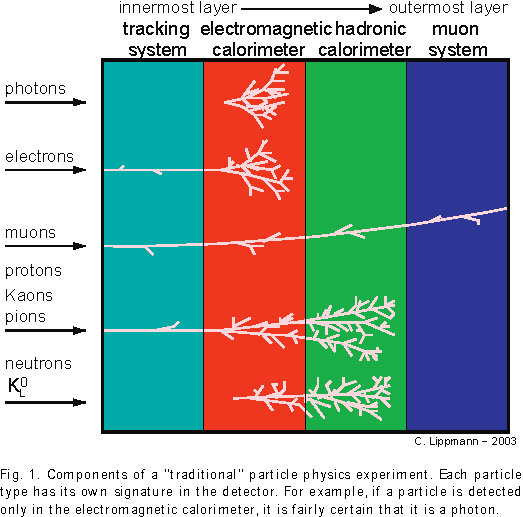
\includegraphics[height=.8\textheight]{plots/particle_signature.pdf}
\end{figure}
\end{frame}


\begin{frame}{particle identification by charge and mass}
\begin{itemize}
\item To identify any stable charged particle, one has to determine its
  \begin{itemize}
  \item charge $ze$, usually $|z|=1$ and sign determined by curvature
  \item mass $m$
  \end{itemize}
\item Mass cannot be directly measured, need other variables $\Rightarrow$ use momentum
\begin{equation}
p=\gamma\beta mc\Longrightarrow m=\frac{p}{\gamma\beta c}
\end{equation}
once velocity is determined, mass is known.
\item 4 ways to determine velocity
  \begin{enumerate}
  \item time of flight
  \item ionization energy loss
  \item Cherenkov
  \item transition radiation
  \end{enumerate}
\end{itemize}
\end{frame}


\begin{frame}{Time-of-flight}
by measuring the particle flight time $t$ over a distance along the track $L$
  \begin{equation}
  \beta=\frac{v}{c}=\frac{L}{tc}
  \end{equation}
  and
  \begin{equation}
  \beta=\frac{1}{\sqrt{\left( \frac{mc}{p} \right)^2+1}}
  \end{equation}
  so
  \begin{equation}
  m=\frac{p}{c}\sqrt{\frac{c^2t^2}{L^2}-1}
  \end{equation}
\end{frame}


\begin{frame}{PHENIX time-of-flight detector (scinllator based)}
\begin{columns}
  \begin{column}{.5\textwidth}
    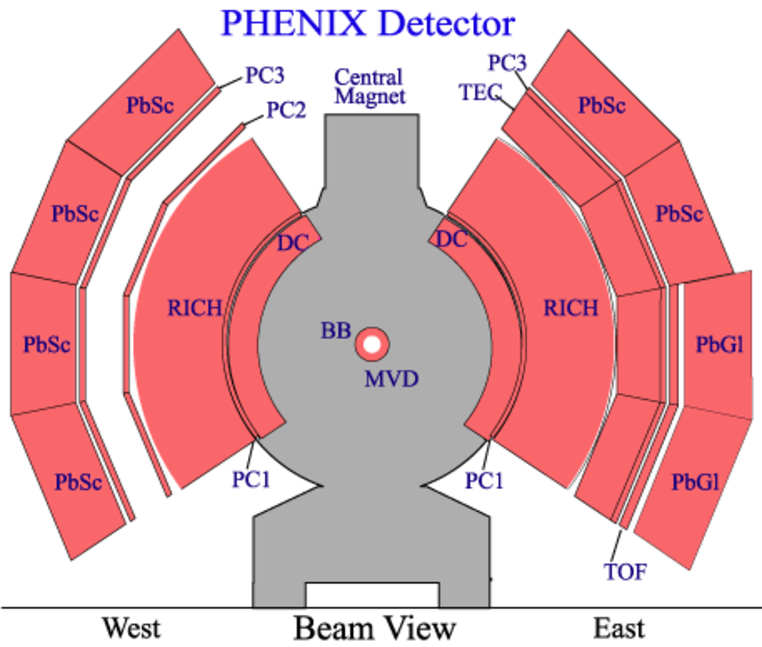
\includegraphics[width=\textwidth]{plots/Phenix_gv.pdf}
  \end{column}
  \begin{column}{.5\textwidth}
    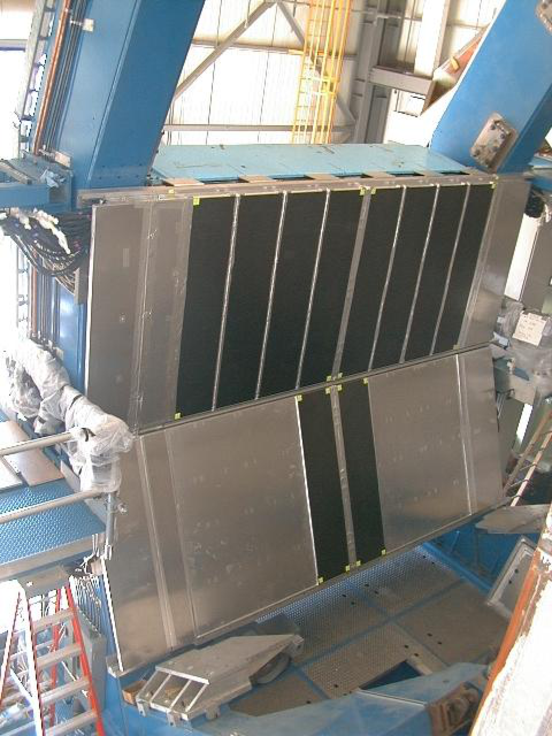
\includegraphics[width=\textwidth]{plots/PHENIX_TOF_panel.pdf}
  \end{column}
\end{columns}
\end{frame}


\begin{frame}{PHENIX particle identification}
  \begin{figure}
    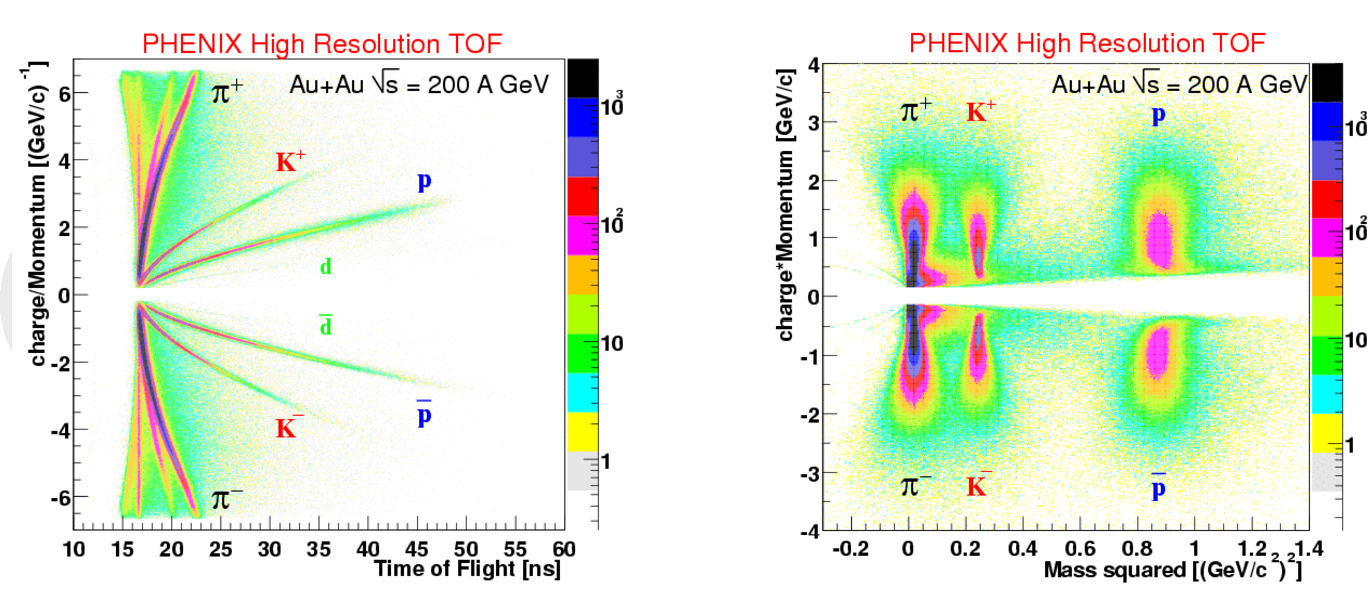
\includegraphics[width=\textwidth]{plots/PHENIX_PID.pdf}
  \end{figure}
  \begin{columns}
    \begin{column}{.5\textwidth}
      \begin{equation*}
        t=\frac{L}{c}\sqrt{1+\left( \frac{mc}{p} \right)^2}
      \end{equation*}
    \end{column}
    \begin{column}{.5\textwidth}
      \begin{equation*}
        m^2=\left( \frac{p}{c} \right)^2 \left( \left( \frac{ct}{L} \right)^2-1 \right)
      \end{equation*}
    \end{column}
  \end{columns}
\end{frame}


\begin{frame}{Resistive Plate Chambers for time-of-flight measurement}
\begin{itemize}
  \item currently scintillators are used due to good time resolution
  \item when experiments scale up, RPCs are simpler and cost effective
\end{itemize}

\begin{columns}
\begin{column}{.6\textwidth}
\begin{figure}
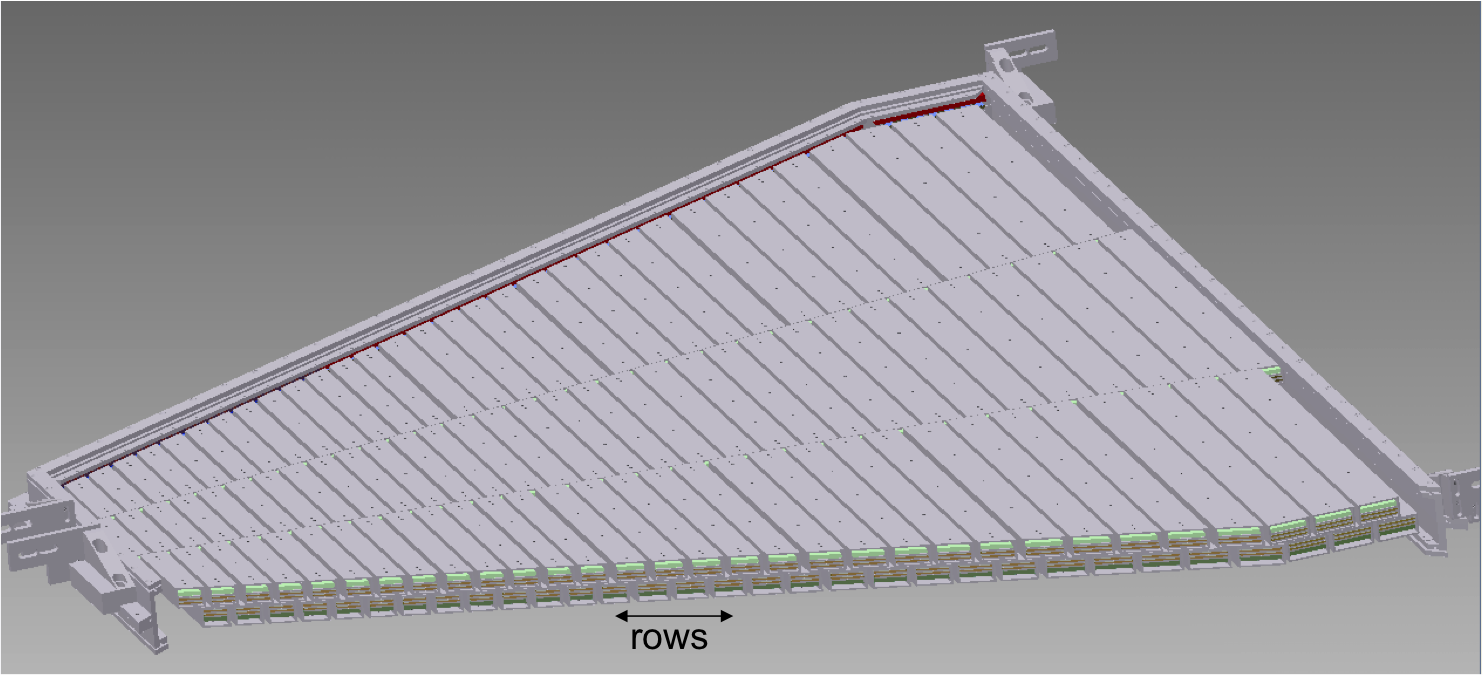
\includegraphics[width=\textwidth]{plots/HADES_RPC.png}
    \caption{TOF Wall of the High Acceptance Di-Electron Spectrometer (HADES)}
\end{figure}
\end{column}
\begin{column}{.4\textwidth}
\begin{figure}
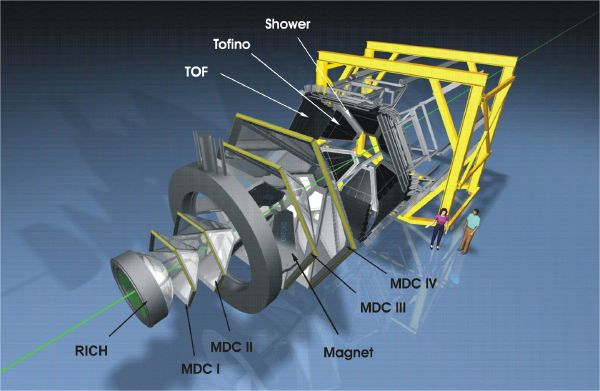
\includegraphics[width=\textwidth]{plots/Hades_scheme.jpg}
\end{figure}
\end{column}
\end{columns}
\end{frame}


\begin{frame}{PID by ionization energy loss}
\begin{itemize}
  \item $\langle dE/dx \rangle$ only depends on velocity, not on particle type
  \item To illustrate, rewrite $\langle dE/dx \rangle$ as a function of $p$
  \begin{equation}
    \left\langle\frac{dE}{dx}\right\rangle=\frac{2\pi NZz^2e^4}{mc^2}\left[ \left( \frac{p^2+M^2c^2}{p^2} \right)  \ln\left( \frac{2p^2m}{IM^2} \right) -1 \right]
  \end{equation}
\end{itemize}
\begin{columns}
  \begin{column}{.5\textwidth}
    \begin{figure}
    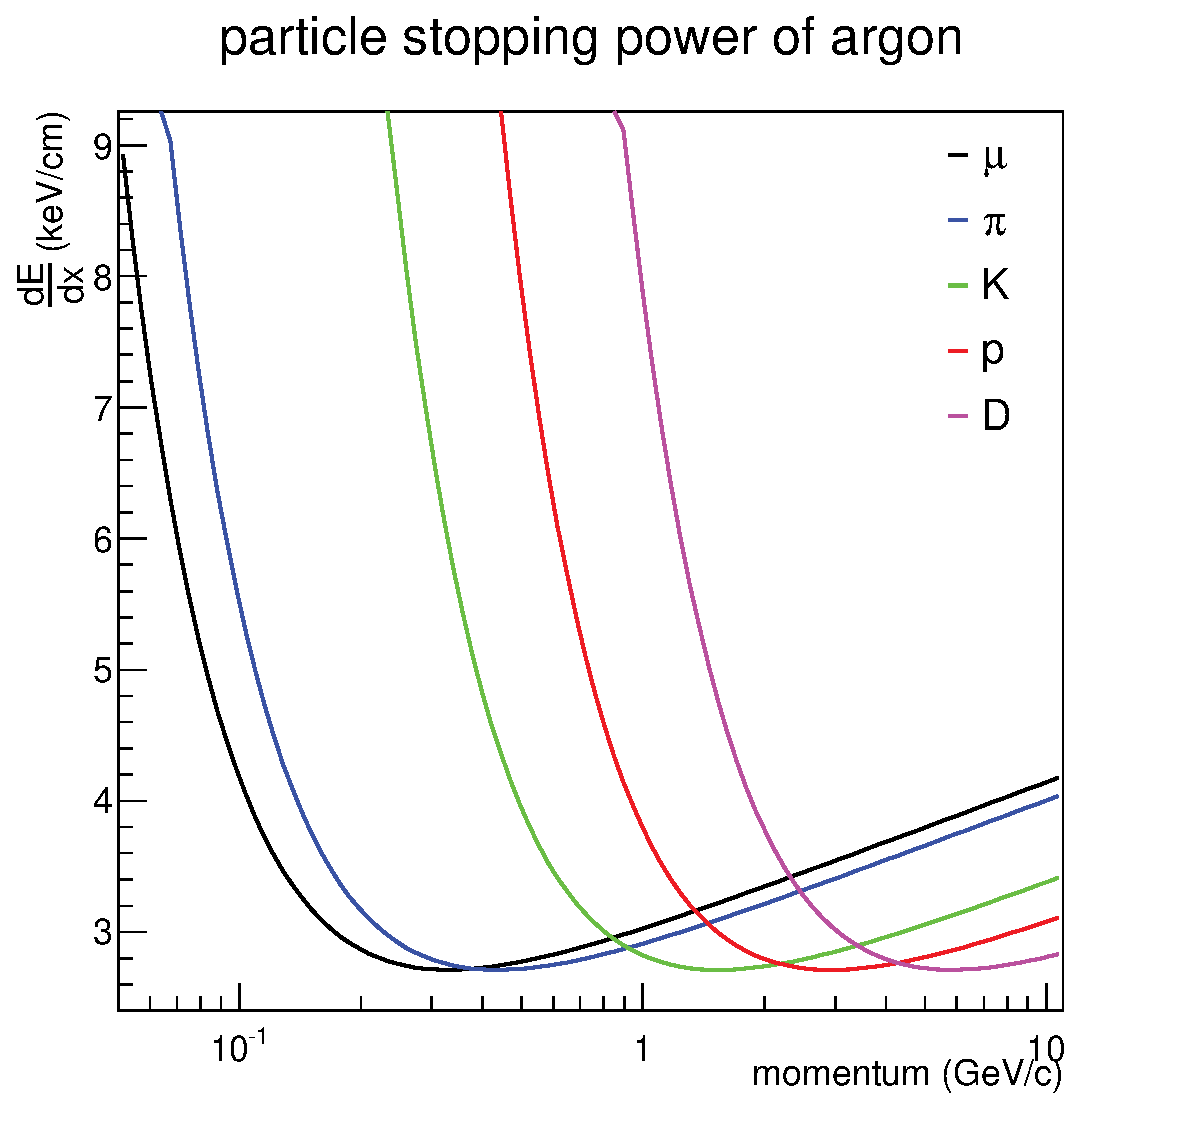
\includegraphics[width=\textwidth]{plots/dEdx.pdf}
    \end{figure}
  \end{column}
  \begin{column}{.5\textwidth}
    \begin{figure}
    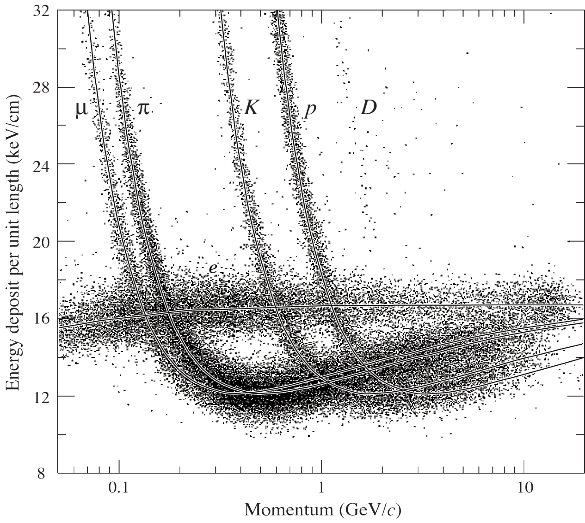
\includegraphics[width=\textwidth]{plots/pep_pid.png}
    \end{figure}
  \end{column}
\end{columns}
\end{frame}


\begin{frame}{Time Projection Chambers (TPC)}
\begin{columns}
\begin{column}{.5\textwidth}
\begin{figure}
  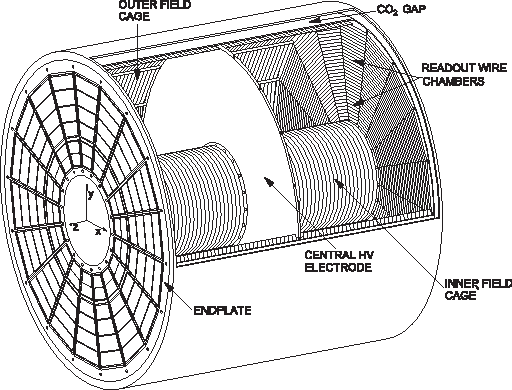
\includegraphics[width=\textwidth]{plots/ALICE_TPC.pdf}
  \caption{3D view of the ALICE TPC field cage}
\end{figure}
\end{column}
\begin{column}{.5\textwidth}
\begin{figure}
  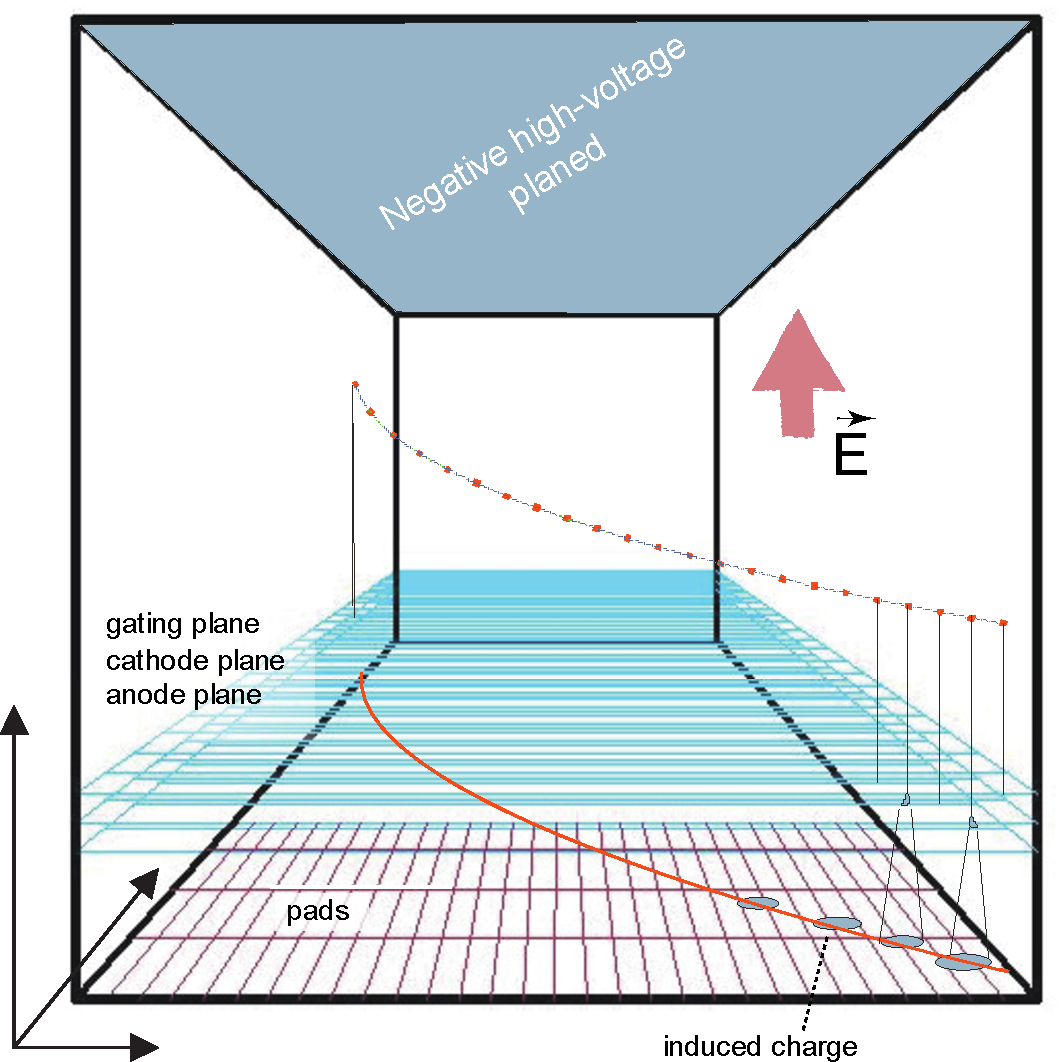
\includegraphics[width=\textwidth]{plots/TPC_cartoon.pdf}
\end{figure}
\end{column}
\end{columns}
\end{frame}



\begin{frame}{centrality measurement}
Why measure centrality?
\begin{itemize}
  \item Centrality is a fundamental characterization of a collision event
  \item Many heavy ion experiment results are presented as functions of centrality  
\end{itemize}
Roadmap to centrality determination
\begin{equation*}
\underbrace{\frac{dN_{ch}}{d\eta}}_{experimental \: observable} \propto \overbrace{\left( N_{coll}, N_{part} \right)}^{modeled\:by\:Glauber} \propto \underbrace{b}_{known\:in\:simulations}\rightarrow centrality
\end{equation*}
\end{frame}


\begin{frame}{Glauber Model}
	\begin{columns}
	\begin{column}{.3\textwidth}
	\begin{figure}
	  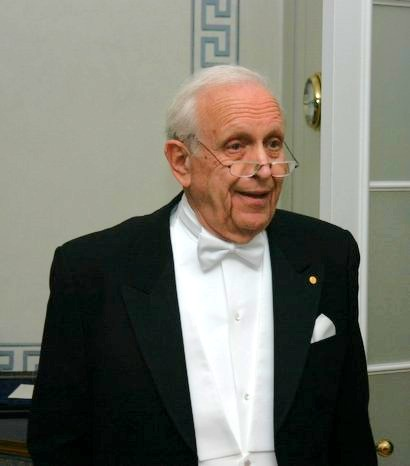
\includegraphics[width=\textwidth]{plots/Roy_Glauber_Dec_10_2005.jpg}
	\end{figure}
	\end{column}
	\begin{column}{.7\textwidth}
	  \begin{itemize}
	    \item proposed by Nobel Laureate Roy Glauber (1925-)
	    \item 2005 Nobel Prize in Physics "for his contribution to the quantum theory of optical coherence"
	    \item controversy: Sudarshan-Glauber representation is based upon the work of Indian physicist George Sudarshan
	  \end{itemize}
	\end{column}
	\end{columns}
	\begin{itemize}
	  \item 1950's: Used quantum mechanical Scattering techniques to analytically describe multi-body scattering of composite systems
	  \item 1970's: Beams of protons and ions were scattered off nuclear targets and Glauber's work was found useful for computing total cross-sections.
	  \item Present: Glauber Montel Carlo Models are used in determining centrality of Heavy Ion Collisions
	\end{itemize}
\end{frame}

\begin{frame}{analytical and Monte Carlo methods}
Two ways: analytical and Monte Carlo
\begin{itemize}
  \item A "True" analytical Glauber Model requires a $2(A+B+1)$ dimensional integral! For Gold thats over 800 dimensions which is very hard to calculate!
  \item Glauber Monte Carlo (GMC): simply count $N_{coll}$ and $N_{part}$
\end{itemize}
\end{frame}


\begin{frame}{Glauber Monte Carlo details: create nuclei}
  \begin{itemize}
    \item The size and shape of nuclei have been determined by electron scattering.
    \item Nucleons in nuclei are modeled by Woods-Saxon distribution
      \scriptsize
      \begin{equation}
      \rho(r,\theta)=\left\{
        \begin{array}{lr}
        \rho_0 \left( \frac{1+w\left(\frac{r}{c}\right)^2}{1+e^x} \right) & \textit{if} \; r<c \\
        \rho_0 \left( \frac{1+w}{1+e^x} \right) & \textit{if} \; r \ge c
        \end{array}
        \right.
      \end{equation}
      \begin{equation}
      \textit{where}\; x=\frac{r-c(1+\beta_{20}Y_{20}(\theta)+\beta_{40}Y_{40}(\theta))}{a(1+\beta_{20}Y_{20}(\theta)+\beta_{40}Y_{40}(\theta))}
      \end{equation}
  \end{itemize}
      The parameters for some relevant nuclei are summarized in the following table%\footnote{\href{http://nuclear.ucdavis.edu/~calderon/Presentations/Phy224C-IntroRHI-Lec7-Glauber_Talk.pdf}{lecture notes by Chris Flores}
      \begin{center}
      \scriptsize
      \begin{tabular}{|c|c|c|c|c|c|c|}
      \hline
       & $\rho_0$ & $w$ & $a$ & $c$ & $\beta_{20}$ & $\beta_{40}$ \\
       \hline
       Au & 0.169 & 0 & 0.535 & 6.38 & -0.131 & -0.031 \\
       \hline
       Pb & 0.1600 & 0 & 0.549 & 6.624 & 0 & 0 \\
       \hline
       Cu & 0.1701 & 0 & 0.586 & 4.214 & 0.162 & -0.006 \\
       \hline
       U & 0.127 & 0.5 & 0.5 & 6.8 & 0.254 & 0.052 \\
       \hline
      \end{tabular}
      \end{center}
\end{frame}


\begin{frame}{Glauber Monte Carlo details}
  \begin{itemize}
    \item \textcolor{cyan}{step 1}: For each nucleon specify a position vector $\vec{p}=(x,y,z)$ drawing from the Woods-Saxon distribution
    \item \textcolor{cyan}{step 2}: Define Orientations of Nuclei and impact parameter $b$
    \begin{itemize}
      \item Generate a random direction on the unit sphere, call it $z'$. Define the rotation from $z$ to $z'$ as $R$.
      \item Draw Random Impact Parameter from Distribution
      \begin{equation}
        d\sigma /db=2\pi b
      \end{equation}
      \item For each nucleon in the projectile nuclei, calculate their position $\vec{p}'=R\vec{p}+(b,0,0)$
    \end{itemize}
  \end{itemize}
\end{frame}


\begin{frame}{Glauber Monte Carlo details}
  \begin{figure}
    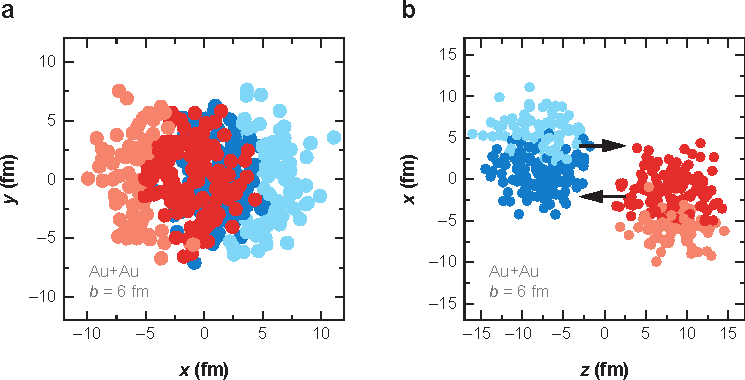
\includegraphics[width=.7\textwidth]{plots/GMC_event.pdf}
  \end{figure}
  \begin{itemize}
    \item \textcolor{cyan}{step 3}: Compute $N_{part}$ and $N_{coll}$ \\
			Define the radius of a nucleon as $r_{nucleon}=\sqrt{\sigma_{NN}/\pi}$
			\begin{enumerate}
			\item if the distance between 2 nucleons $d_{NN}<2r_{nucleon}$, increment $N_{coll}$.
			\item if $N_{coll}>0$, increment $N_{part}$.
			\end{enumerate}
  \end{itemize}
\end{frame}


\begin{frame}{Glauber Monte Carlo results}
  \begin{figure}
    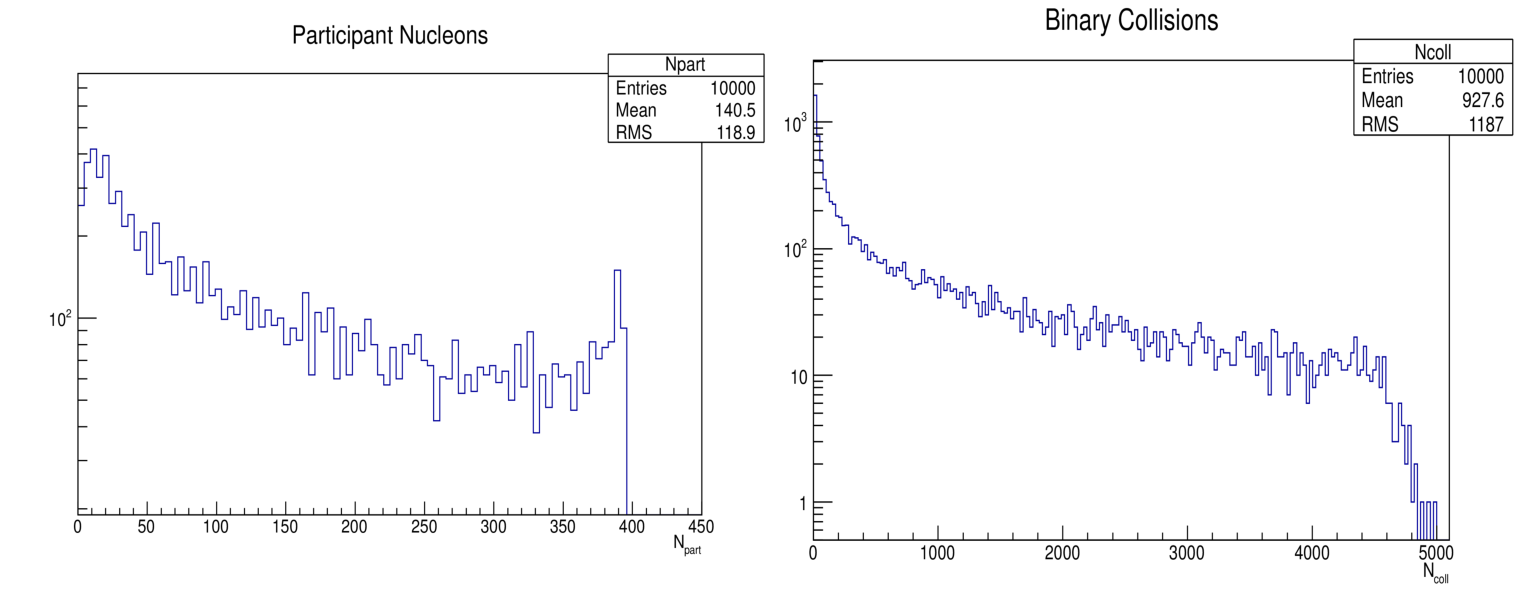
\includegraphics[width=\textwidth]{plots/GMC_results.pdf}
  \end{figure}
  \begin{equation*}
    \% \:central=\frac{b}{R_A+R_B}
  \end{equation*}
\end{frame}


\begin{frame}{PHENIX beam-beam counter (BBC)}
  \begin{figure}
    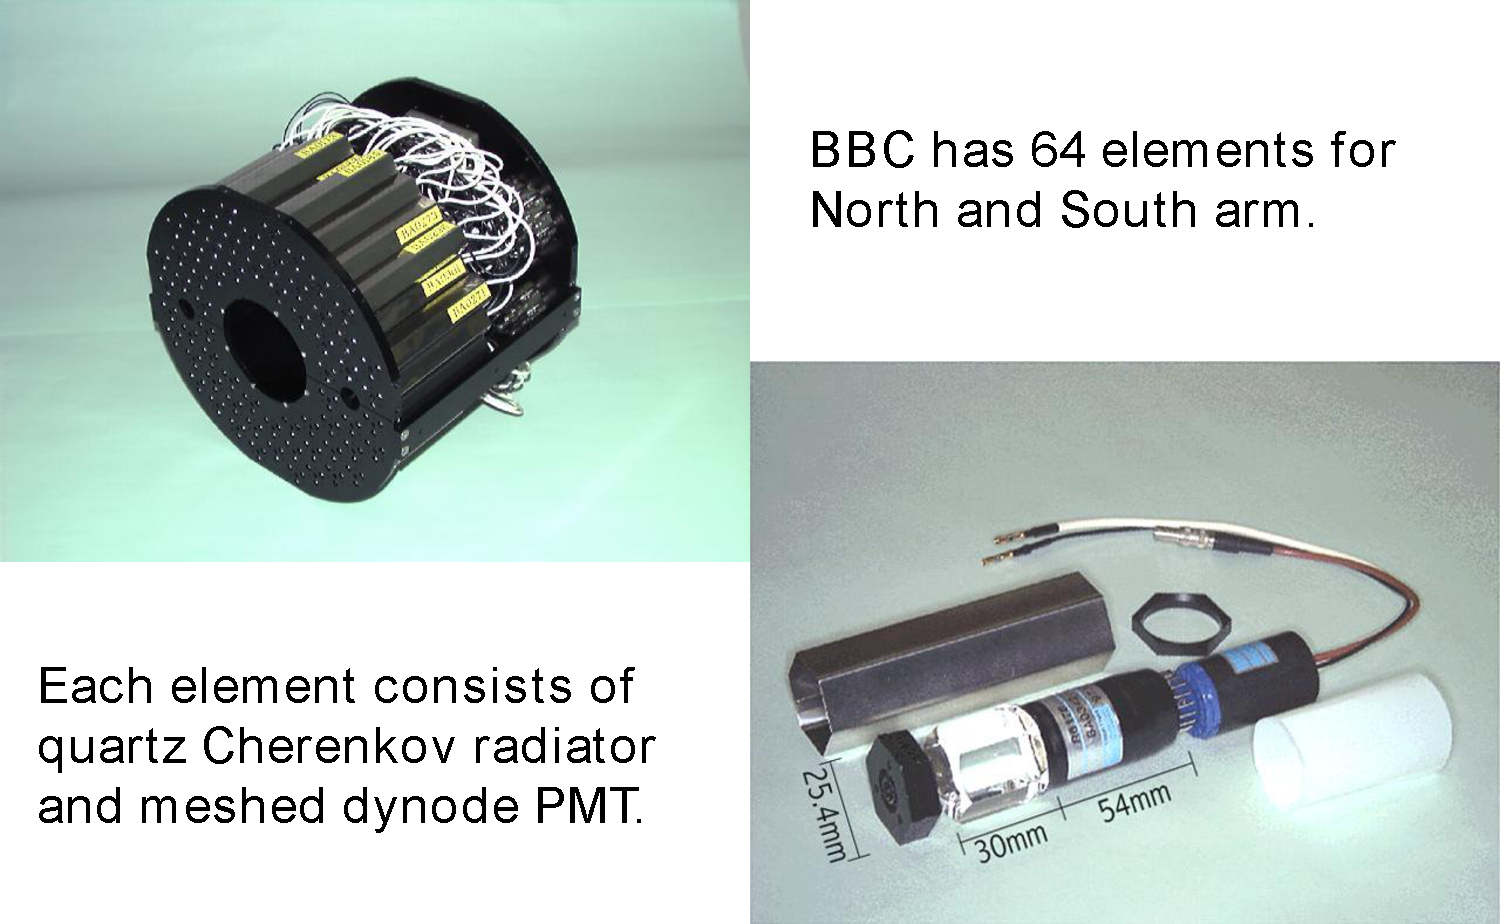
\includegraphics[width=\textwidth]{plots/BBC_component.pdf}
  \end{figure}
\end{frame}


\begin{frame}{purpose of PHENIX BBC}
  \begin{figure}
    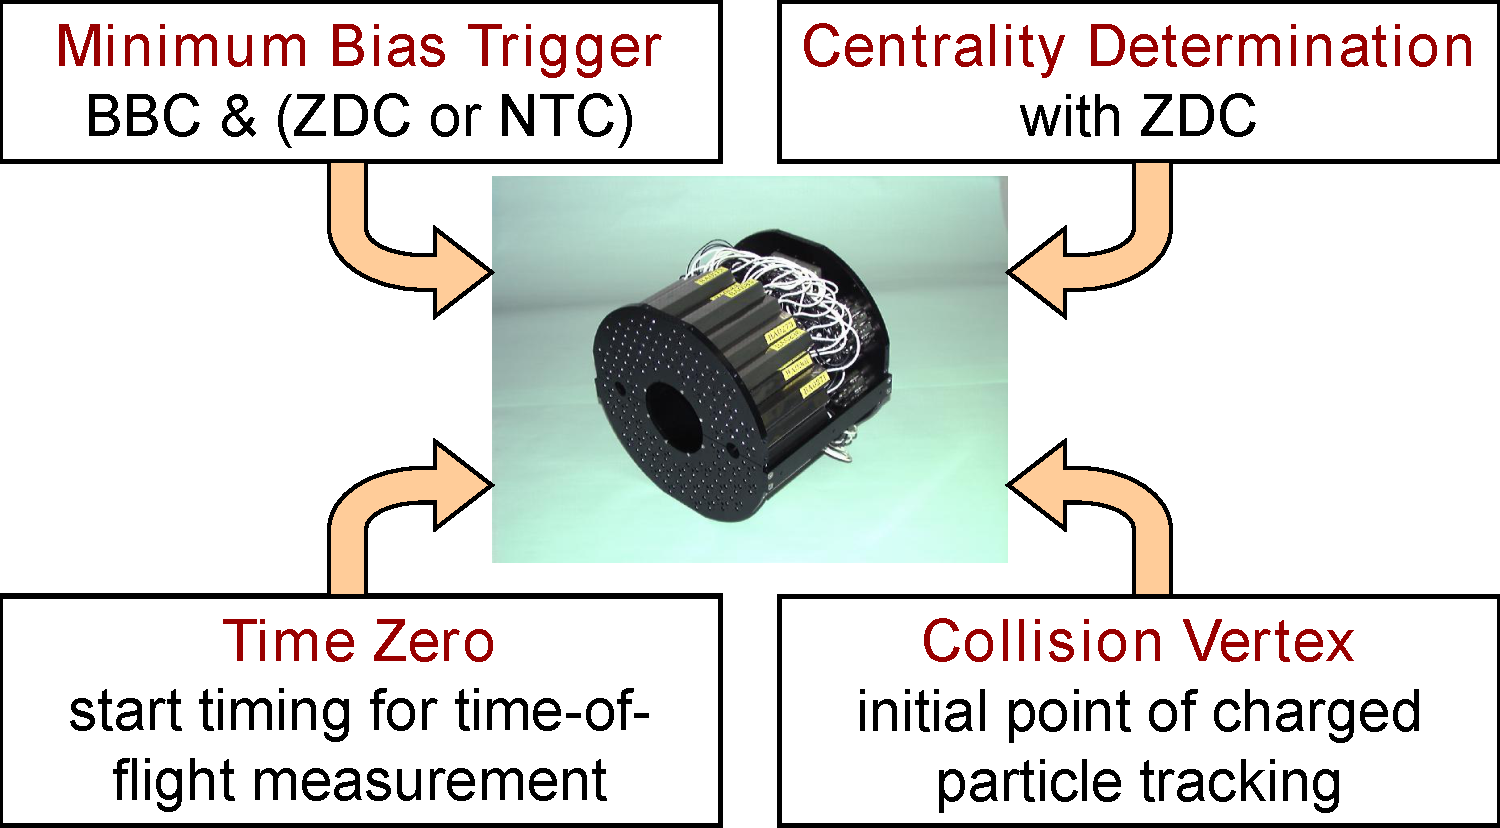
\includegraphics[width=\textwidth]{plots/PHENIX_BBC_purpose.pdf}
  \end{figure}
\end{frame}



\begin{frame}{PHENIX BBC location}
  \begin{figure}
    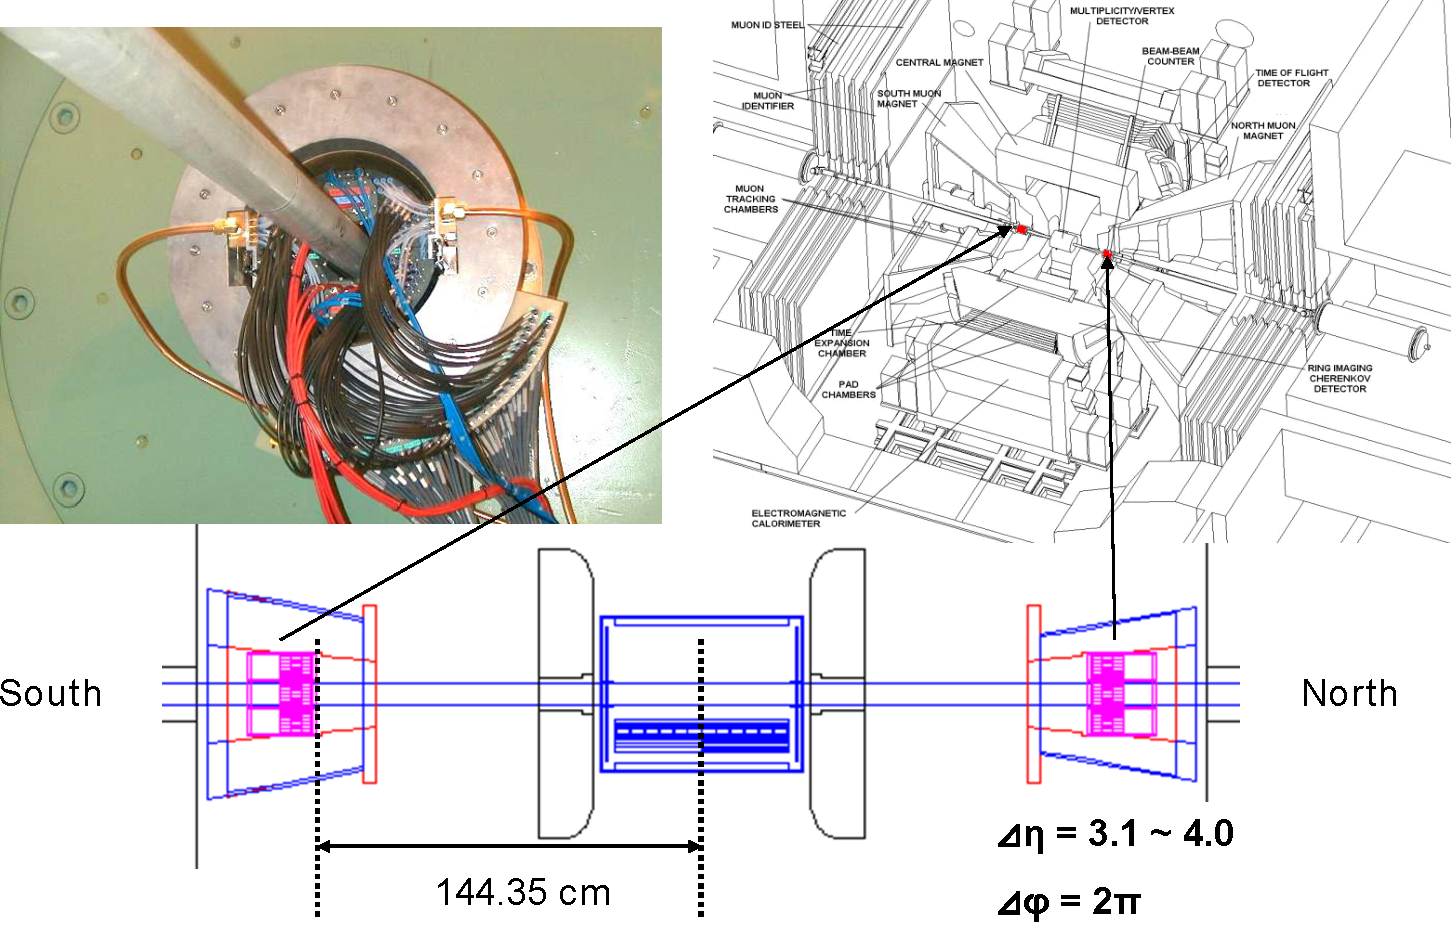
\includegraphics[width=\textwidth]{plots/PHENIX_BBC_location.pdf}
  \end{figure}
\end{frame}


\begin{frame}{from BBC hits to $N_{part}$: negative binomial distribution}
  \begin{itemize}
    \item It is found the BBC $N_{hit}$ spectrum is well described by the negative binomial distribution (NBD)
    \begin{equation}
		NBD(N_{part},\mu,k)=\frac{\Gamma(N_{part}+k)}{\Gamma(k)N_{part}!}\left( \frac{\mu}{k} \right)^{N_{part}}\frac{1}{(1+\mu/k)^{N_{part}+k}}
		\end{equation}
		here $\mu=\langle N_{part}\rangle$ and $k$ is related to the width of the distribution.
		
		\item Denote the GMC $N_{part}$ spectrum by $GMC(N_{part})$, the BBC $N_{hit}$ spectrum can be written as
		\begin{equation}\label{eq:bbcformula}
		BBC(N_{hit})=\epsilon(N_{hit})\sum\limits_{N_{part}}NBD(N_{part},\mu,k)\times GMC(N_{part})
		\end{equation}
		where $\epsilon(N_{hit})$ is the BBC detection efficiency.
  \end{itemize}
\end{frame}


\begin{frame}{construct the $N_{hit}\rightarrow N_{part}\rightarrow b$ lookup table}
  \begin{columns}
    \begin{column}{.5\textwidth}
      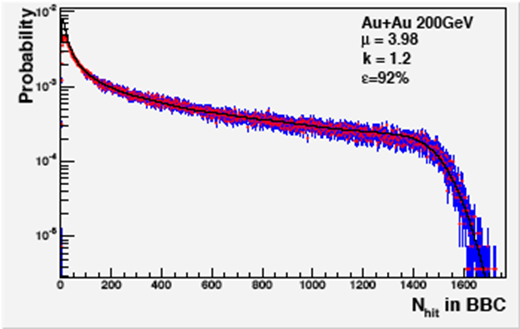
\includegraphics[width=\textwidth]{plots/Nhit_BBC.png}
    \end{column}
    \begin{column}{.5\textwidth}
      \begin{itemize}
        \item By fitting BBC $N_{hit}$ spectrum to equation (\ref{eq:bbcformula}), one gets parameters $\mu$ and $k$.
      \end{itemize}
    \end{column}
  \end{columns}
  \begin{itemize}
      \item Once $\mu$ and $k$ are known, for a given $N_{part}$ value one can get the mean value of $N_{hit}$. Then we have $N_{hit}\rightarrow N_{part}$.
      \item For a given $b$, one can get the mean value of $N_{part}$. Then we have $N_{part}\rightarrow b$. Therefore we have $N_{hit}\rightarrow N_{part}\rightarrow b$.
    \end{itemize}
\end{frame}



\begin{frame}{temperature measurement}
Q: How to measure the initial temperature of QGP?\\
A: Through thermal photons.\\
QGP information is carried by direct photons since they interact weakly with the medium.
\begin{itemize}
  \item What are direct photons?\\
  Direct photons are photons directly produced in scattering processes, not from decays (e.g. neutral pions)
  \item two kinds of direct photons:
  \begin{enumerate}
    \item prompt photons, produced in hard scattering, high $p_T$
    \item thermal photons, produced in thermal production, low $p_T$
  \end{enumerate}
\end{itemize}
\end{frame}


\begin{frame}{direct photon examples\footnote{Annu. Rev. Nucl. Part. Sci. 2005. 55:517-54}}
  \begin{figure}
    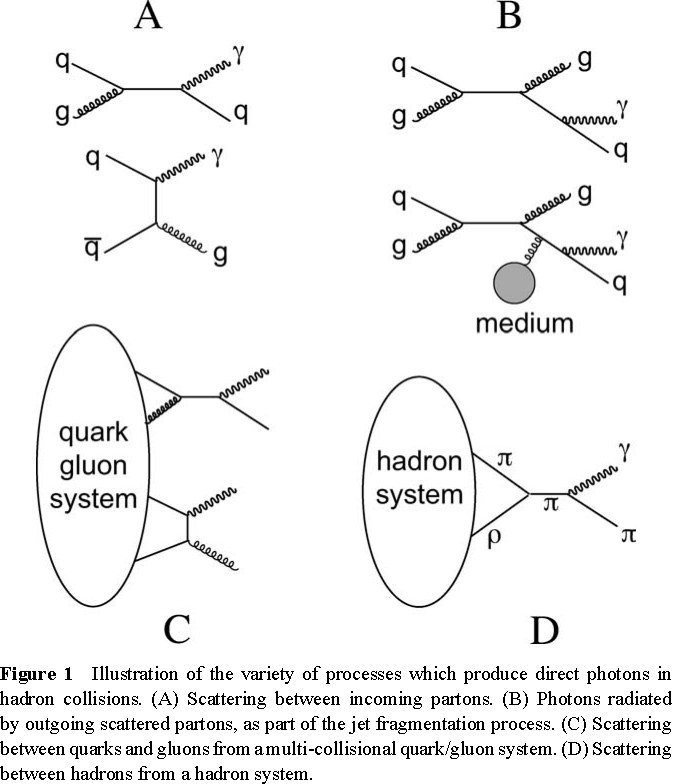
\includegraphics[height=.8\textheight]{plots/direct_photon_examples.pdf}
  \end{figure}
\end{frame}



\begin{frame}{fitting PHENIX data}
  \begin{columns}
    \begin{column}{.4\textwidth}
    \begin{figure}
      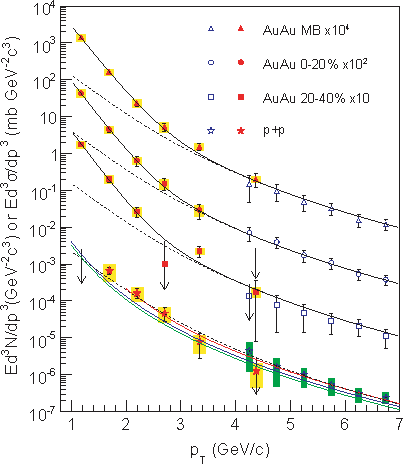
\includegraphics[width=\textwidth]{plots/direct_photon_spectrum.pdf}
      \caption{invariant yield of direct photons}    
    \end{figure}
    \end{column}
    \begin{column}{.6\textwidth}
      \scriptsize
      \begin{itemize}
        \item To circumvent the limitations due to the energy resolution at low photon energies, the di-electron channel (e.g. $qg\rightarrow \gamma^*g\rightarrow e^+e^-g$) is used.
        \item $p+p$ data match LNO pQCD calculation(solid lines) quite well and goes like modified power law
        \begin{equation}
				\frac{A_{pp}}{\left( 1+\frac{p_T}{b} \right)^n}
				\end{equation}
				\item In low $p_T$ region, the yield of $Au+Au$ rises faster than $p+p$ scaled by $T_{AA}\sim \langle N_{coll}\rangle$.
				\item Thus by fitting to
				\begin{equation}
				Ae^{-\frac{p_T}{T}}+T_{AA}\frac{A_{pp}}{\left( 1+\frac{p_T}{b} \right)^n}
				\end{equation}
				a temperature for central collision of $T=221\pm 19^{stat} \pm 19^{syst}$ MeV is obtained.
      \end{itemize}
    \end{column}
  \end{columns}
\end{frame}



\begin{frame}{summary}
  \begin{itemize}
    \item A heuristic derivation of Bethe's formula is discussed.
    \item Several ways to identify particles are presented.
    \item Centrality measurement is discussed from experimental observables to Glauber Monte Carlo modeling.
    \item Temperature measurement is discussed.
  \end{itemize}
\end{frame}

\end{document}